%%%%%%%%%%%%%%%%%%%%%%%%%%%%%%%%%%%%%%%%%%%%%%%%%%%%%%%%%%%%%%%
%
% Welcome to writeLaTeX --- just edit your LaTeX on the left,
% and we'll compile it for you on the right. If you give
% someone the link to this page, they can edit at the same
% time. See the help menu above for more info. Enjoy!
%
%%%%%%%%%%%%%%%%%%%%%%%%%%%%%%%%%%%%%%%%%%%%%%%%%%%%%%%%%%%%%%%

% --------------------------------------------------------------
% This is all preamble stuff that you don't have to worry about.
% Head down to where it says "Start here"
% --------------------------------------------------------------
 
\documentclass[12pt]{report}
 
\usepackage[margin=1in]{geometry}
\usepackage{amsmath,amsthm,amssymb}
\usepackage{hyperref}
\usepackage[nottoc,numbib]{tocbibind}
\usepackage{graphicx}
\graphicspath{{./images/}}

\usepackage{tikz}
\usetikzlibrary{shapes,positioning}

\tikzset{ell/.style={circle,draw,minimum height=0.5cm,minimum width=0.5cm,inner sep=0.2cm}}
\tikzset{rec/.style={rectangle,draw,minimum height=0.5cm,minimum width=0.5cm,inner sep=0.2cm}}

\usepackage{listings}
\usepackage{xcolor}

%New colors defined below
\definecolor{codegreen}{rgb}{0,0.6,0}
\definecolor{codegray}{rgb}{0.5,0.5,0.5}
\definecolor{codepurple}{rgb}{0.58,0,0.82}
\definecolor{backcolour}{rgb}{0.95,0.95,0.92}

%Code listing style named "mystyle"
\lstdefinestyle{mystyle}{
  backgroundcolor=\color{backcolour}, commentstyle=\color{codegreen},
  keywordstyle=\color{magenta},
  numberstyle=\tiny\color{codegray},
  stringstyle=\color{codepurple},
  basicstyle=\ttfamily\footnotesize,
  breakatwhitespace=false,         
  breaklines=true,                 
  captionpos=b,                    
  keepspaces=true,                 
  numbers=left,                    
  numbersep=5pt,                  
  showspaces=false,                
  showstringspaces=false,
  showtabs=false,                  
  tabsize=2
}

%"mystyle" code listing set
\lstset{style=mystyle}

 
\newcommand{\N}{\mathbb{N}}
\newcommand{\Z}{\mathbb{Z}}
 
\newenvironment{theorem}[2][Theorem]{\begin{trivlist}
\item[\hskip \labelsep {\bfseries #1}\hskip \labelsep {\bfseries #2.}]}{\end{trivlist}}
\newenvironment{lemma}[2][Lemma]{\begin{trivlist}
\item[\hskip \labelsep {\bfseries #1}\hskip \labelsep {\bfseries #2.}]}{\end{trivlist}}
\newenvironment{exercise}[2][Exercise]{\begin{trivlist}
\item[\hskip \labelsep {\bfseries #1}\hskip \labelsep {\bfseries #2.}]}{\end{trivlist}}
\newenvironment{problem}[2][Problem]{\begin{trivlist}
\item[\hskip \labelsep {\bfseries #1}\hskip \labelsep {\bfseries #2.}]}{\end{trivlist}}
\newenvironment{question}[2][Question]{\begin{trivlist}
\item[\hskip \labelsep {\bfseries #1}\hskip \labelsep {\bfseries #2.}]}{\end{trivlist}}
\newenvironment{corollary}[2][Corollary]{\begin{trivlist}
\item[\hskip \labelsep {\bfseries #1}\hskip \labelsep {\bfseries #2.}]}{\end{trivlist}}

\newenvironment{solution}{\begin{proof}[Solution]}{\end{proof}}
 
\begin{document}
 
% --------------------------------------------------------------
%                         Start here
% --------------------------------------------------------------
 
\title{Texas A\&M University Kingsville\\
Department of EECS\\
CSEN 5303 Foundations of Computer Science\\
Project 3 Sorting
}%Institution, Department
\author{\\
Mengxiang Jiang\\ %replace with your name
Professor Habib Ammari} %if necessary, replace with your course title
 
\maketitle

\tableofcontents

\chapter{Introduction}
The problem given is to sort an array containing the characters `A', `M', and `T',
 such that all the $T's$ appear first, followed by all the $A's$, and lastly all the $M's$.
Special constraints are in place to make this sort harder:
\begin{quote}
\textbf{-Constraint 1:} Each letter (`A', `M', or `T') is evaluated \textbf{only once}.\\
\textbf{-Constraint 2:} The function $SWAP(TAM,i,j)$ is \textbf{used only} when it is \textbf{necessary}.\\
\textbf{-Constraint 3: No extra space} can be used by the algorithm $Sort\_TAM$. In other words,
\textbf{only} the array TAMUK can be used to sort the `A', `M', or `T'.\\
\textbf{-Constraint 4:} You \textbf{cannot count} the number of each letter `A', `M', or `T'.
\end{quote}
The main algorithm used is a type of insertion sort, and the programming language used to implement it is Python.
\chapter{Design}
\label{chapter:design}
First I will show the algorithm in pseudocode and then give a short example of how it works.
Here is the pseudocode:
\begin{verbatim}
procedure Sort_TAM(TAMUK: arrayChar);
    var
        last_t, first_m, i: integer;
    begin
        last_t := -1;
        first_m := n;
        i := 0;
        while (i < first_m) do
            if TAMUK[i] = 'M' then
                while (TAMUK[first_m - 1] = 'M') do
                    first_m := first_m - 1;
                if i < first_m - 1 then
                    SWAP(TAMUK, i, first_m - 1);
                    first_m := first_m - 1;
            if TAMUK[i] = 'T' then
                if i > last_t + 1 then
                    SWAP(TAMUK, i, last_t + 1);
                last_t := last_t + 1;
            i := i + 1;
    end;
\end{verbatim}
\pagebreak
Suppose the given character array, $TAMUK$, is given as below:\\\\
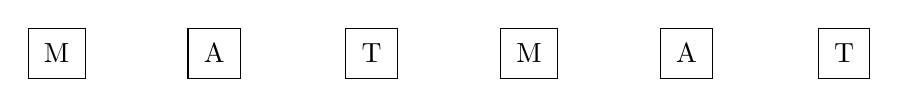
\begin{tikzpicture}[>=stealth]
    \node[rec] (m1) at (0,0) {M};
    \node[rec] (a1) at (2,0) {A};
    \node[rec] (t1) at (4,0) {T};
    \node[rec] (m2) at (6,0) {M};
    \node[rec] (a2) at (8,0) {A};
    \node[rec] (t2) at (10,0) {T};
\end{tikzpicture}
\\We initialize our variables: $last\_t=-1$ and $first\_m=6$\\\\
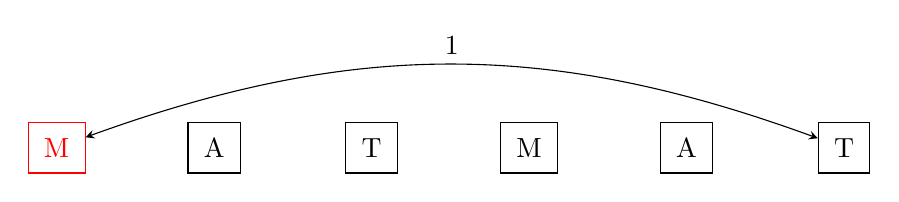
\begin{tikzpicture}[>=stealth]
    \node[red,rec] (m1) at (0,0) {M};
    \node[rec] (a1) at (2,0) {A};
    \node[rec] (t1) at (4,0) {T};
    \node[rec] (m2) at (6,0) {M};
    \node[rec] (a2) at (8,0) {A};
    \node[rec] (t2) at (10,0) {T};
    \draw [<->] (m1) to [bend left=20]node[above]{$1$} (t2);
\end{tikzpicture}
\\We evaluate $TAMUK[0]$: $last\_t=0$ and $first\_m=5$\\\\
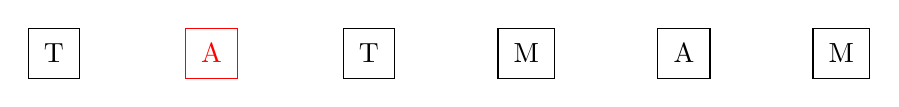
\begin{tikzpicture}[>=stealth]
    \node[rec] (t2) at (0,0) {T};
    \node[red,rec] (a1) at (2,0) {A};
    \node[rec] (t1) at (4,0) {T};
    \node[rec] (m2) at (6,0) {M};
    \node[rec] (a2) at (8,0) {A};
    \node[rec] (m1) at (10,0) {M};
\end{tikzpicture}
\\We evaluate $TAMUK[1]$: $last\_t=0$ and $first\_m=5$\\\\
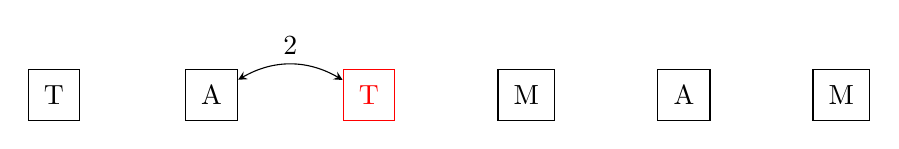
\begin{tikzpicture}[>=stealth]
    \node[rec] (t2) at (0,0) {T};
    \node[rec] (a1) at (2,0) {A};
    \node[red,rec] (t1) at (4,0) {T};
    \node[rec] (m2) at (6,0) {M};
    \node[rec] (a2) at (8,0) {A};
    \node[rec] (m1) at (10,0) {M};
    \draw [<->] (t1) to [bend right]node[above]{$2$} (a1);
\end{tikzpicture}
\\We evaluate $TAMUK[2]$: $last\_t=1$ and $first\_m=5$\\\\
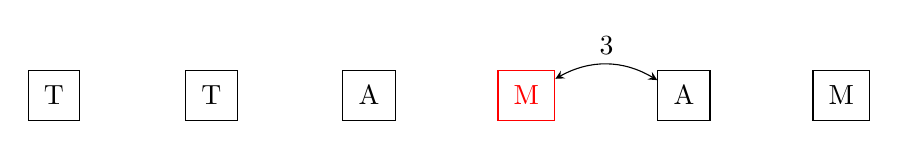
\begin{tikzpicture}[>=stealth]
    \node[rec] (t2) at (0,0) {T};
    \node[rec] (t1) at (2,0) {T};
    \node[rec] (a1) at (4,0) {A};
    \node[red,rec] (m2) at (6,0) {M};
    \node[rec] (a2) at (8,0) {A};
    \node[rec] (m1) at (10,0) {M};
    \draw [<->] (m2) to [bend left]node[above]{$3$} (a2);
\end{tikzpicture}
\\We evaluate $TAMUK[3]$: $last\_t=1$ and $first\_m=4$\\\\
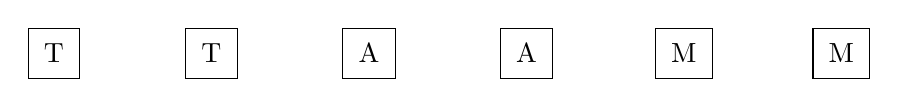
\begin{tikzpicture}[>=stealth]
    \node[rec] (t2) at (0,0) {T};
    \node[rec] (t1) at (2,0) {T};
    \node[rec] (a1) at (4,0) {A};
    \node[rec] (a2) at (6,0) {A};
    \node[rec] (m2) at (8,0) {M};
    \node[rec] (m1) at (10,0) {M};
\end{tikzpicture}
\\Since $first\_m=4$, we don't need to evaluate $TAMUK[4]$ and can stop, so this is the final sorted array.\\\\
This algorithm is correct since it is insertion sort with an improvement. 
Rather than doing a maximum of $O(n)$ swaps in order to place the current element in the intermediate sorted list, 
it is able to place it in a maximum of 2 swaps. Thus, the worst case run time is $O(n)$ rather than $O(n^2)$ for standard insertion sort.
The reason only 2 swaps maximum is needed is that we keep track of the position of the last known letter $T$ and the position of the first known letter $M$, 
and only need to swap to these two locations (with their respective offsets) for the current element.

\chapter{Code}
\begin{lstlisting}[language=Python, caption=sort\_tam.py]
"""
class for sorting an array of T's, A's, and M's
"""

class SortTAM:
    def __init__(self, tam):
        self.tamuk = [c for c in tam]
        # if the last character in the string is '#', remove from array
        if self.tamuk[-1] == '#':
            self.tamuk = self.tamuk[:-1]
    
    # sorts the tamuk array
    def sort_tam(self):
        last_t = -1
        first_m = len(self.tamuk)
        i = 0
        while(i < first_m):
            if self.tamuk[i] == 'M':
                while(self.tamuk[first_m - 1] == 'M'):
                    first_m -= 1
                if i < first_m - 1:
                    self.swap(i, first_m - 1)
                    first_m -= 1
            if self.tamuk[i] == 'T':
                if i > last_t + 1:
                    self.swap(i, last_t + 1)
                last_t += 1
            i += 1
    # swaps elements in the i-th and j-th position of the array tamuk
    def swap(self, i, j):
        self.tamuk[i], self.tamuk[j] = self.tamuk[j], self.tamuk[i]


def main():
    raw_input = input("Please enter a string of T's, A's, and M's in any order (i.e. MMAATT):")
    st = SortTAM(raw_input)
    st.sort_tam()
    print(f'The sorted string is {"".join(st.tamuk)}')

if __name__ == '__main__':
    main()
\end{lstlisting}

\begin{lstlisting}[language=Python, caption=sort\_tam\_gui.py]
import tkinter as tk
from sort_tam import SortTAM

def display_sort_tam():
    given_tam = tam_entry.get()
    st = SortTAM(given_tam)
    st.sort_tam()
    given_label["text"] = f"Given String: {given_tam}"
    sorted_label["text"] = f"Sorted String: {''.join(st.tamuk)}"

window = tk.Tk()
tam_label = tk.Label(text="Enter String of T's, A's, and M's")
tam_entry = tk.Entry()
enter_button = tk.Button(text="Submit", command=display_sort_tam)
given_label = tk.Label(text="Given String:")
sorted_label = tk.Label(text="Sorted String:")
tam_label.pack()
tam_entry.pack()
enter_button.pack()
given_label.pack()
sorted_label.pack()
window.mainloop()
\end{lstlisting}

\begin{figure}[ht]
    \centering
    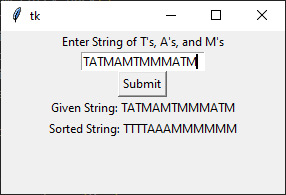
\includegraphics[]{gui}
    \caption{gui}
\end{figure}

\chapter{Tests}
\begin{lstlisting}[language=Python, caption=sort\_tam\_tests.py]
import unittest
from sort_tam import SortTAM

class TestSortTAM(unittest.TestCase):
    # test already sorted
    def test_already_sorted(self):
        tam = 'TTAAAMMMM'
        st = SortTAM(tam)
        st.sort_tam()
        self.assertEqual(''.join(st.tamuk), tam)
    
    #test a string with all 3 types of letters
    def test_normal(self):
        tam = 'ATMTTAMMAM'
        st = SortTAM(tam)
        st.sort_tam()
        self.assertEqual(''.join(st.tamuk), 'TTTAAAMMMM')
    
    #test a string with only Ts and Ms
    def test_tm(self):
        tam = 'MTMMMTTTMTM'
        st = SortTAM(tam)
        st.sort_tam()
        self.assertEqual(''.join(st.tamuk), 'TTTTTMMMMMM')
    
    #test a string with only As and Ms
    def test_am(self):
        tam = 'AMMMAAMAMAM'
        st = SortTAM(tam)
        st.sort_tam()
        self.assertEqual(''.join(st.tamuk), 'AAAAAMMMMMM')
    
    #test a string with only As and Ts
    def test_at(self):
        tam = 'ATAATATTATA'
        st = SortTAM(tam)
        st.sort_tam()
        self.assertEqual(''.join(st.tamuk), 'TTTTTAAAAAA')

if __name__ == '__main__':
    unittest.main()
\end{lstlisting}

\chapter{Lessons Learned}
I initially had an algorithm that swapped the letter $A$ around, but the resulting number of swaps was much more than the minimum needed. 
I learned some graph theory in order to merge the swaps in order to get to the minimum, 
but the solution would have used extra space to store the swaps, which meant it violated constraint 3 and therefore was not good enough.
I then went to Professor Ammari's office hours and showed him the algorithm and asked for any suggestions and improvements.
With his help, I got to the algorithm currently used. So the big lesson I learned was to not be afraid to ask for help when you are stuck.
\bibliographystyle{plain}
\bibliography{refs}

% --------------------------------------------------------------
%     You don't have to mess with anything below this line.
% --------------------------------------------------------------
 
\end{document}